\chapter{Introducción}

La \textbf{Robo R2} es una impresora 3D de tipo FDM (modelado por deposición fundida): funde filamento plástico y construye la pieza capa por capa. Este manual resume, para uso en el laboratorio, lo esencial del manual del fabricante~\cite{robomanual}: cómo ponerla en marcha, calibrarla, imprimir una pieza, controlarla a distancia y mantenerla en buen estado.

El flujo de trabajo es siempre el mismo: se diseña o descarga un modelo (\texttt{.stl}), un programa \textbf{laminador} (Cura for Robo) lo convierte en instrucciones (\texttt{.gcode}) y la impresora las ejecuta desde su pantalla táctil, una memoria USB o el panel web.

\begin{figure}[H]
    \centering
    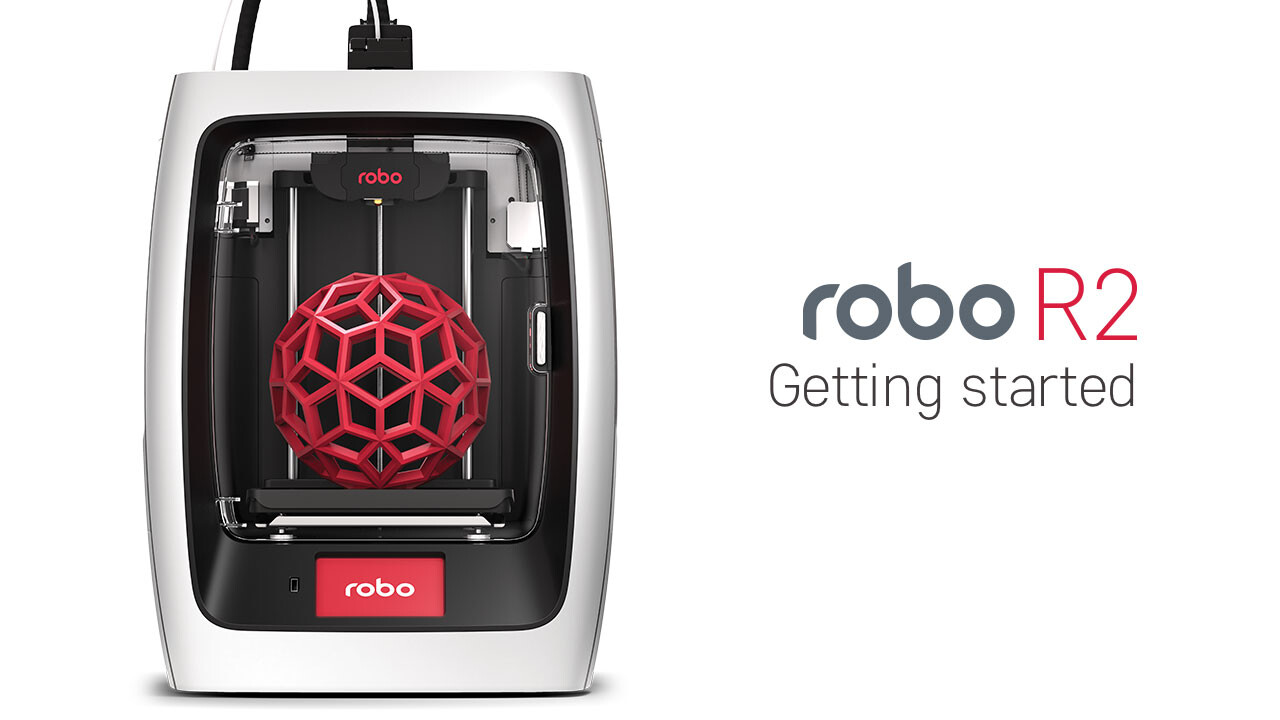
\includegraphics[width=0.55\linewidth]{r2_inicio.jpg}
    \caption{Impresora Robo R2 (imagen del manual del fabricante~\cite{robomanual}).}
    \label{fig:r2}
\end{figure}

\section{Contenido de la caja}

Además de la impresora, la caja incluye:

\begin{itemize}
    \item Guía de inicio rápido y voucher de un año del software Autodesk Fusion~360.
    \item Fuente de alimentación de 24~V y tubo guía del filamento.
    \item Caja de herramientas: tapa del hotend, 2 llaves allen, lubricante, pinzas y tarjeta de calibración del Z-Offset.
    \item Memoria USB de Robo, 300~g de filamento (celeste) y espátula.
\end{itemize}

\begin{figure}[H]
    \centering
    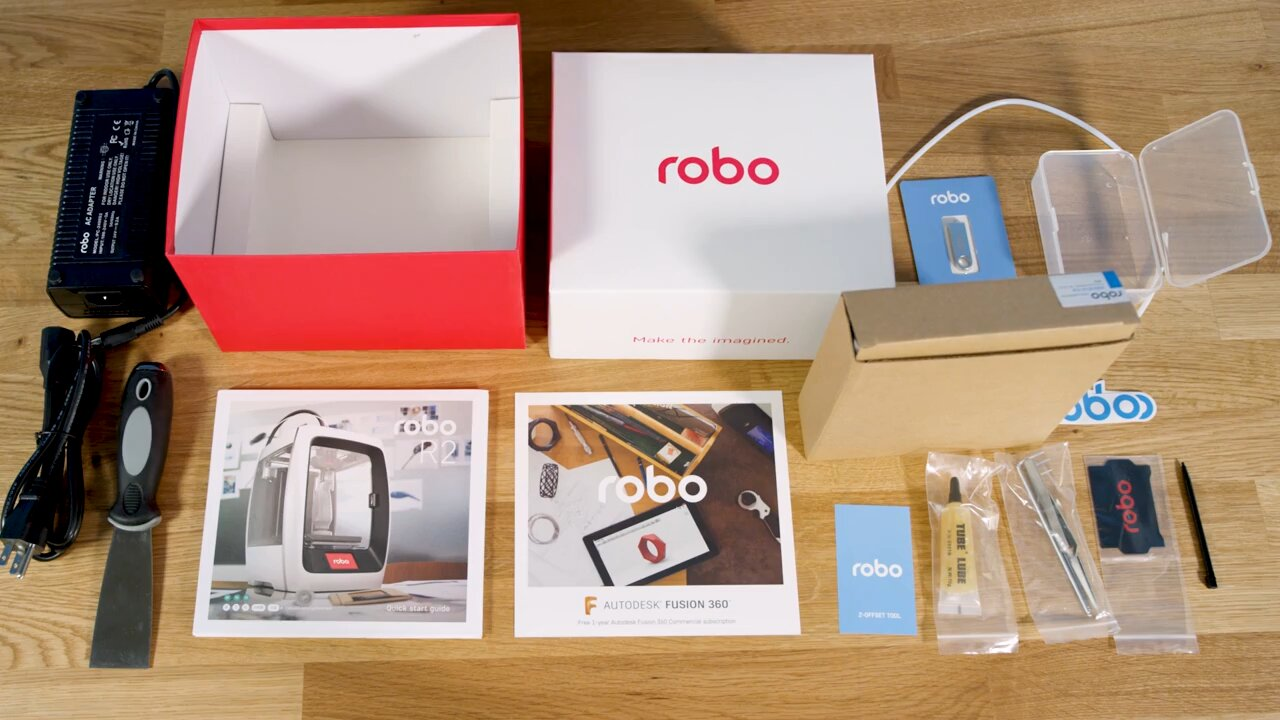
\includegraphics[width=0.7\linewidth]{r2_caja.jpg}
    \caption{Accesorios que vienen con la impresora.}
    \label{fig:caja}
\end{figure}

\section{La pantalla táctil}

La pantalla táctil a color es el punto de acceso principal: se maneja con el dedo o con un lápiz táctil. Tiene tres pestañas:

\begin{description}[leftmargin=2.2cm,style=nextline]
    \item[Files] Archivos de la memoria interna o de una USB.
    \item[Printer] Pantalla de impresión: archivo en curso, temperaturas, progreso, mensajes de error y botones Pause y Cancel.
    \item[Utilities] Ventiladores, asistentes (Wizards), red, actualización y opciones.
\end{description}

\begin{figure}[H]
    \centering
    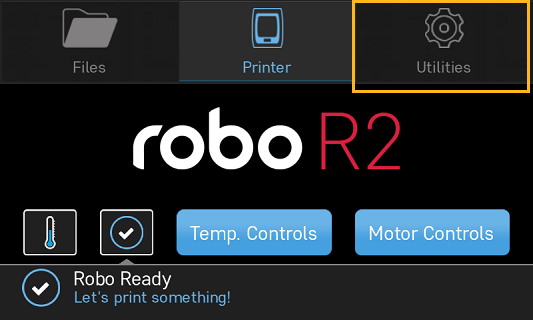
\includegraphics[width=0.48\linewidth]{r2_pantalla_inicio.png}\hfill
    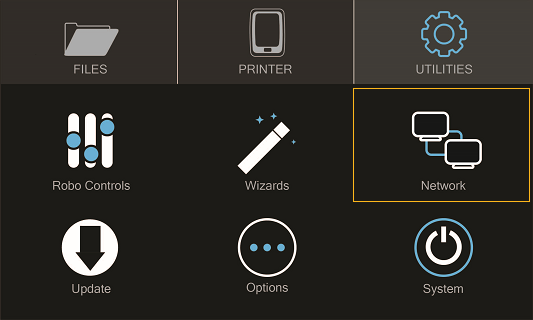
\includegraphics[width=0.48\linewidth]{r2_utilities.png}
    \caption{Pantalla de inicio (izquierda) y menú \emph{Utilities} (derecha).}
    \label{fig:pantallas}
\end{figure}

\section{Seguridad}

\begin{warningbox}[Lea esto antes de usar la impresora]
\begin{itemize}
    \item \textbf{Quemaduras:} el hotend puede llegar a unos \grados{300} y la cama a unos \grados{110}. No toque el hotend con las manos; si es necesario, use las pinzas y espere al menos 30 minutos a que se enfríe.
    \item \textbf{Partes móviles:} no meta la mano ni objetos dentro de la impresora cuando esté en marcha, a punto de arrancar o en reposo.
    \item \textbf{No la deje sola} durante una impresión y apáguela al terminar.
    \item \textbf{Electricidad:} use solo el cable original, con buena conexión a tierra. Todo mantenimiento se hace con la impresora apagada y desenchufada. No modifique la electrónica.
    \item \textbf{Ventilación:} el plástico fundido emite olor; trabaje en un lugar ventilado. No ponga comida ni bebida cerca.
    \item Use guantes al retirar las piezas y las herramientas solo para su fin. Mantenga el equipo lejos de líquidos, fuentes de calor y de niños.
\end{itemize}
\end{warningbox}

\section{Estructura del manual}

\begin{itemize}
    \item \textbf{Práctica 1:} puesta en marcha y calibración.
    \item \textbf{Práctica 2:} preparación e impresión de una pieza.
    \item \textbf{Práctica 3:} control remoto con panel web, app y cámara.
    \item \textbf{Capítulo 5:} mantenimiento y solución de problemas.
\end{itemize}
